\documentclass[12pt,a4paper]{article}
\usepackage{fullpage}
\usepackage[margin=1.5cm]{geometry}
\usepackage{amsmath}
\usepackage{subfig}
\usepackage{graphicx}
\usepackage[justification=centering]{caption}
\usepackage{enumitem}
\usepackage{multirow}

\begin{document}
\title{Training model on others input of pronotum datasets}
\author{LE Van Linh}
\date{\today}
\maketitle
\begin{abstract}
	In this study, we use the network model that we had submitted to ICPRS-18 to find the results on the new size of the input images. Instead of using the images with the size of $256 \times 192$, we have chosen a ``square" size for the images. The new sizes of images which used to study are $224 \times 224$ and $96 \times 96$. The model will be trained on each dataset in $10000$ epochs. The experiments will be compared the losses during training, statistic analysis and time-consuming. In the context of this study, we used term \textbf{``the last result"} to mention the result what we have submitted to ICPRS-18.
\end{abstract}
\section{Introduction}
In the last result, we have proposed a network to predict the landmarks on pronotum images. It receives an image of $1 \times 256 \times 192$ as the input. The network was constructed from $3$ \textit{``elementary block"} following by $3$ full-connected layers. An elementary block is defined as a sequence of convolution $(C_i)$, pooling $(P_i)$ and dropout $(D_i)$ layers. The parameters for each layers are as below, the list of values follows the order of elementary blocks:
\begin{itemize}[nosep,label=\footnotesize$\bullet$]
	\item CONV layres:
	\begin{itemize}[nosep]
		\item Number of filters: 32, 64 and 128,
		\item Kernel filters size: $(3 \times 3), (2 \times 2)$, and $(2 \times 2)$
		\item Stride values: $1,1,1$
		\item No padding is used for CONV layers
	\end{itemize}
	\item POOL layers:
	\begin{itemize}[nosep]
		\item Kernel filters size: $(2 \times 2), (2 \times 2)$, and $(2 \times 2)$
		\item Stride values: $2,2,2$
		\item No padding is used for CONV layers
	\end{itemize}
	\item DROP layers:
	\begin{itemize}
		\item Propabilities: $0.1, 0.2$ and $0.3$.
	\end{itemize}
\end{itemize}
In the last full-connected layers (FC), the parameters are: FC1
output: $1000$, FC2 output: $1000$, FC3 output: $16$. As usual, a
dropout layer is inserted between FC1 ond FC2 with a probability equal to $0.5$. Fig.\ref{cnnnetwork2} illustrate the order of the layers in the network.

\begin{figure*}[h]
\centering
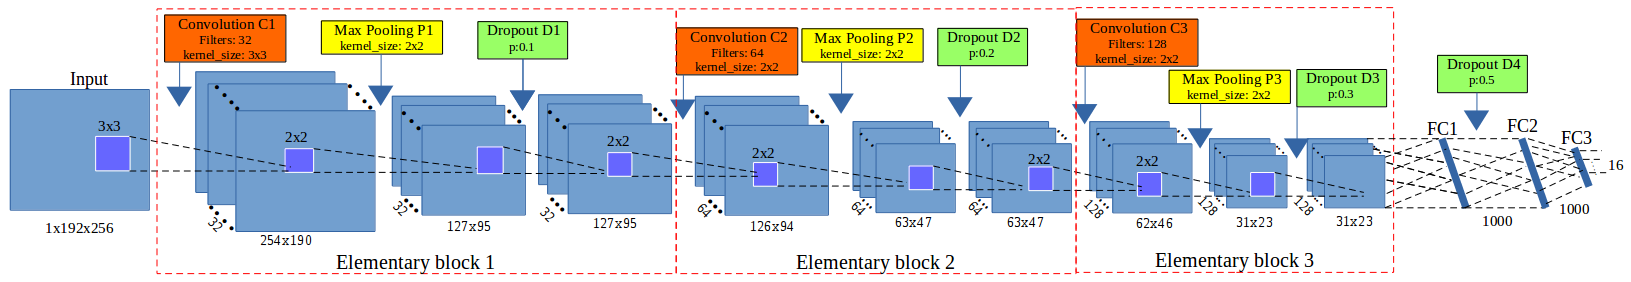
\includegraphics[scale=0.32]{images/cnn_newdatasize/arch_model}
\caption{{\small{Network architecture using $3$ \textit{elementary blocks}.
  Convolution
  layer in red, pooling in yellow and dropout in green color.}}} 
\label{cnnnetwork2}
\end{figure*}

In our study, instead of using a \textit{``square"} image, we have used a \textit{``rectangle"} image as the input. The result shows that the network has the ability to work well on the input that size of width and height are different. Considering as a different of workflows, we would like to see how the network works on ``square" input. In this study, we continue train the proposed network () on $2$ new dataset with different size: $224 \times 224$ and $96 \times 96$.

\section{Dataset}
The dataset includes 293 RGB-images of beetle's pronotum. The images were taken by the same camera with the same conditions of resolution of $3264 \times 2448$. The images in the dataset were divided into two subsets: training (including $260$ images) and testing (including $33$ images). For each image, a set of 8 manual landmarks have been set by biologists.
In this section, we introduce the process to down-sample the original images to the new size of images. Then, we augment the images for training and validation (it have been presented in ICPRS-18).
\subsection{DATA\_1: size of $224 \times 224$}
To obtain a new size of the input image ($224 \times 224$) from the original image, we have applied procedure as followed: Firstly, the images are down-sampled to a resolution of $326 \times 245$ and the coordinates of the manual landmarks are also re-scaled. Secondly, the centroid point of manual landmarks is calculated for each image. The centroid point is considered as the center of the new image that has been cropped from the down-sampled image. The size of the new image is fixed as $224 \times 224$. From the centroid point, we expand in four directions of the image until satisfying the size. Then, the coordinates of manual landmarks are re-calculated to fit with the new image. Fig. \ref{figdata} presents an example in dataset after down-sampling and crop the image to fit with the input size of the neural network.

\begin{figure}[h!]
\centering
\subfloat[]{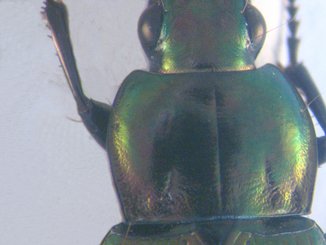
\includegraphics[scale=1.1]{./images/imagenet_finetuning/Prono_001_326}\label{a1}}\hspace{1cm}
\subfloat[]{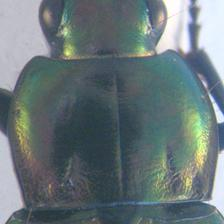
\includegraphics[scale=0.5]{./images/imagenet_finetuning/Prono_001_224}{\label{a2}}}
\caption{An example in dataset. \textit{a)} presents the image after down-sampling. \textit{b)} presents the cropped image from down-sampling image which used as the input of CNN}
\label{figdata}
\end{figure}

\subsection{DATA\_2: size of $96 \times 96$}
In the other side, to obtain the images size of $96 \times 96$, we have applied the procedure following:
\begin{enumerate}[nosep]
	\item Left crop image to obtain the new size of $2448 \times 2448$,
	\item Down-sample the image to size of $96 \times 96$,
	\item Scale the coordinates of the manual landmarks to adapt with the new size of images.
\end{enumerate}

\section{Experiments}
The proposed network has been trained on two datasets with different of input size: $224 \times 224$ and $96 \times 96$ in $10000$ epochs. We have applied cross-validation to obtain fully the prediction of landmarks of all images. Table.\ref{tab2} shows losses during training on each round.
For dataset of $224 \times 224$ images, the average loss of validation stage (RMSE) is \textit{$sqrt(0.0000767) \times 112 = 0.981$} pixels; while, this value for dataset of $96 \times 96$ is \textit{$sqrt(0.00004) \times 48 = 0.00192$} pixels.

\begin{table}[htbp]
\centering
\begin{tabular}{ | c | c | c | c | c | }
\hline
	\multicolumn{1}{|c|}{\multirow{2}{*}{Round}} & \multicolumn{2}{c|}{$224 \times 224$} &  \multicolumn{2}{c|}{$96 \times 96$}  \\ \cline{2-5}
	 & Train loss & Validation loss & Train loss & Validation loss \  \\ \hline
	\textbf{1} & \textbf{0.00012} & \textbf{0.00009} & \textbf{0.00015} & \textbf{0.00004} \\ \hline
	2 & 0.00012 & 0.00006 & 0.00015 & 0.00004 \\ \hline
	3 & 0.00012 & 0.00007 & 0.00015 & 0.00006 \\ \hline
	4 & 0.00012 & 0.00009 & 0.00015 & 0.00004 \\ \hline
	5 & 0.00013 & 0.00010 & 0.00016 & 0.00005 \\ \hline
	\textbf{6} & \textbf{0.00012} & \textbf{0.00006} & \textbf{0.00014} & \textbf{0.00003} \\ \hline
	7 & 0.00013 & 0.00008 & 0.00014 & 0.00003 \\ \hline
	8 & 0.00012 & 0.00006 & 0.00015 & 0.00004 \\ \hline
	9 & 0.00013 & 0.00008 & 0.00014 & 0.00003 \\ \hline
\end{tabular}
\caption{\small{A comparing of losses during training between the datasets.}}
\label{tab2}
\end{table}

Table.\ref{tab3} shows the average distances in pixels and standard deviation (SD) when we calculate the distance from the coordinates of predicted landmarks to coordinates of manual landmarks.
\begin{table}[htbp]
\centering
\begin{tabular}{ | c | c | c | c | c | }
\hline
	\multicolumn{1}{|c|}{\multirow{2}{*}{Landmark}} & \multicolumn{2}{c|}{$224 \times 224$} &  \multicolumn{2}{c|}{$96 \times 96$}  \\ \cline{2-5}
	 & Avg distance & SD & Avg distance & SD \  \\ \hline
	\textbf{1} & \textbf{3.2974} & \textbf{2.2689} & \textbf{1.6136} & \textbf{0.9332
} \\ \hline
	2 & 3.9845 & 2.6562 & 1.8399 & 1.1190 \\ \hline
	3 & 3.4676 & 2.3424 & 1.6248 &	1.0027 \\ \hline
	4 & 3.8779 & 2.7883 & 1.8787	& 1.2135 \\ \hline
	5 & 3.5482 & 2.5824 & 1.7616 &	1.1022 \\ \hline
	\textbf{6} & \textbf{4.2235} & \textbf{3.2746} & \textbf{2.1340} &\textbf{1.3440} \\ \hline
	7 & 3.3834 & 2.3783 & 1.6150 &	1.0217 \\ \hline
	8 & 4.0352 & 2.8116 & 1.9779 &	1.2735 \\ \hline	
\end{tabular}
\caption{\small{A comparing of average distance and SD on two dataset.}}
\label{tab3}
\end{table}


\section{Conclusions}
In this study, we have trained the model on pronotum dataset but the size of images are changed to $224 \times 224$ and $96 \times 96$. This study shows that the losses during training are the same with the last one, but we have a difference about the average distance among the results on each dataset. Additional, when we training with small input, the training time had improved than with the large input.
\bibliographystyle{unsrt}
\bibliography{includes/references}

\end{document}